\chapter{Results and Discussion}
\label{results}

In this thesis, parameters of node2vec and edge2vec are optimized to generate best performance classification models. Then comparison between learned features and engineered features are conducted by replacing engineered feature vectors with learned feature vectors generated by node2vec and edge2vec. Furthermore, the chosen models are used to predict novel drug-disease edges. The below paragraphs demonstrate results of comparisons and predictions.

\section{A Comparison Between Engineered and Learned Features}

For comparing the performances of classification models trained by learned features and engineered features, the first step is to optimize the parameters of node2vec and edge2vec to generate high-quality feature vectors. After the parameter optimization, comparisons are conducted between the chosen models and Rephetio's. 


\subsection{Parameter Optimization of Node2vec and Comparisons}

As discussed in section \ref{op_node2vec} and \ref{op_edge2vec}, dimensions, \textot{num$\_$walks}, \textit{walk$\_$length}, \textit{p}, \textit{q} and operator are optimized sequentially in this thesis. First of all, the \ac{AUC-ROC} is chosen to evaluate the models trained by learned features and then parameters are selected based on evaluations.

The fisrt optimized parameter is \textit{dimensions}, As illustrated in Figure \ref{fig:dimensions}, \textit{dimensions} is changed from 16, 32, 48, 64, 159. The \ac{AUC-ROC}s drop to 0.5 when $dimensions = 64$, but return to similar values with $dimensions = 32, 48$ when $dimensions = 159$, which doesn't mean 64 dimensions is not suitable for this method because it may be caused by the randomness of node2vec and edge2vec during random walk. Even though, this result is meaningful in which it shows that node2vec and hetionet is not sensitive to \textit{dimensions}. Since smaller \textit{dimensions} has comparable performance with larger \textit{dimensions}, the smaller one 64 is chosen for avoiding overfitting.

\begin{figure}[!h]
    \centering
    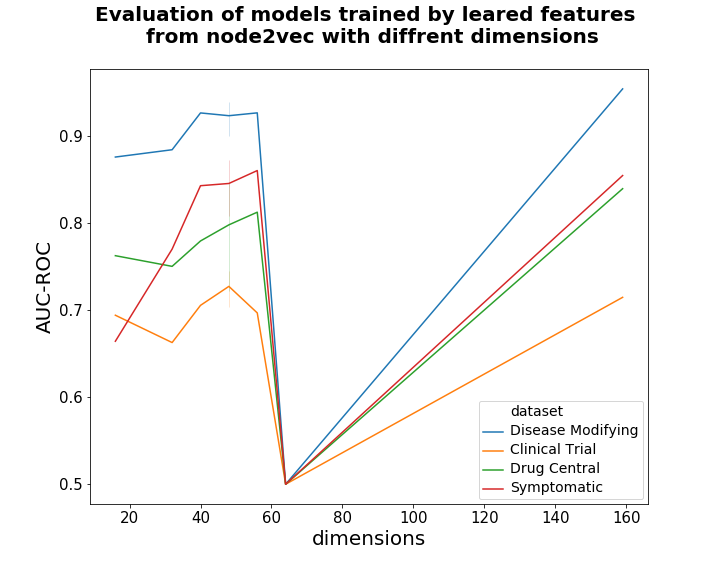
\includegraphics[scale=0.55]
    {figures/dimensions.png}
    \captionsetup{justification=centering}
    \caption[Evaluation of different dimensions in node2vec]{\label{fig:dimensions}Performance of logistic regression models with parameters: $p = 1$, $q = 1.0$. $repeat = 1$, $walk\_length = 30$, $window\_size = 10$, $number\_walk = 10$, $dimensions = 16, 32, 48, 64, 159$ Star signs are values of Rephetio.
}
\end{figure}

The randomness challenges the process of parameter optimization when the results fluctuate with same parameters. The next step is to control the effects of randomness by tuning relative parameters. In node2vec and edge2vec, the core model is skip-gram, whose actual training data is 'walks' generated by random walk. If the random walk is operated for more times, the training data should be more comprehensive and representative for the network. Then \textit{num$\_$walks} is tested with 10, 20, 30. Surprisingly, among all repeated experiments with same other parameters except \textit{num$\_$walks}, $num\_walks = 10$ gives 90\% valid models (logistic regression models trained by learned features from node2vec whose evaluation results are not 0.5), $num\_walks = 20$ giving 40\% ones, and $num\_walks = 30$ giving 40\% ones too. The reason of such results might be that the hetionet is a complexed network, when \textit{num$\_$walks} gets larger, the 'walks' becomes more diverse and sparse for the skip-gram model. Then the logistic regression models fail with low-quality learned features. Also, it was reported that node2vec can catch useful structure information of network with small \textit{num$\_$walk}. At last, $num\_walks = 10$ is chosen.

Another important parameter is \textit{window size}, which controls distance of nodes affecting the center node in walks in node2vec scenario. For evaluating the results properly, 10 repeated experiments are operated with same parameters to reduce the confusion from randomness. 2, 6, 10 are tried in this thesis. As illustrated in Figure \ref{fig:window_size}, the average of AUC-ROC values get better when \textit{window size} gets larger for Drug Central and Symptomatic. For Clinical Trial, the results of $window size = 2, 6, 10$ are similar but $window size = 10$ makes the performance of models more stable. $window size = 10$ is chosen at last. 

\begin{figure}[!h]
    \centering
    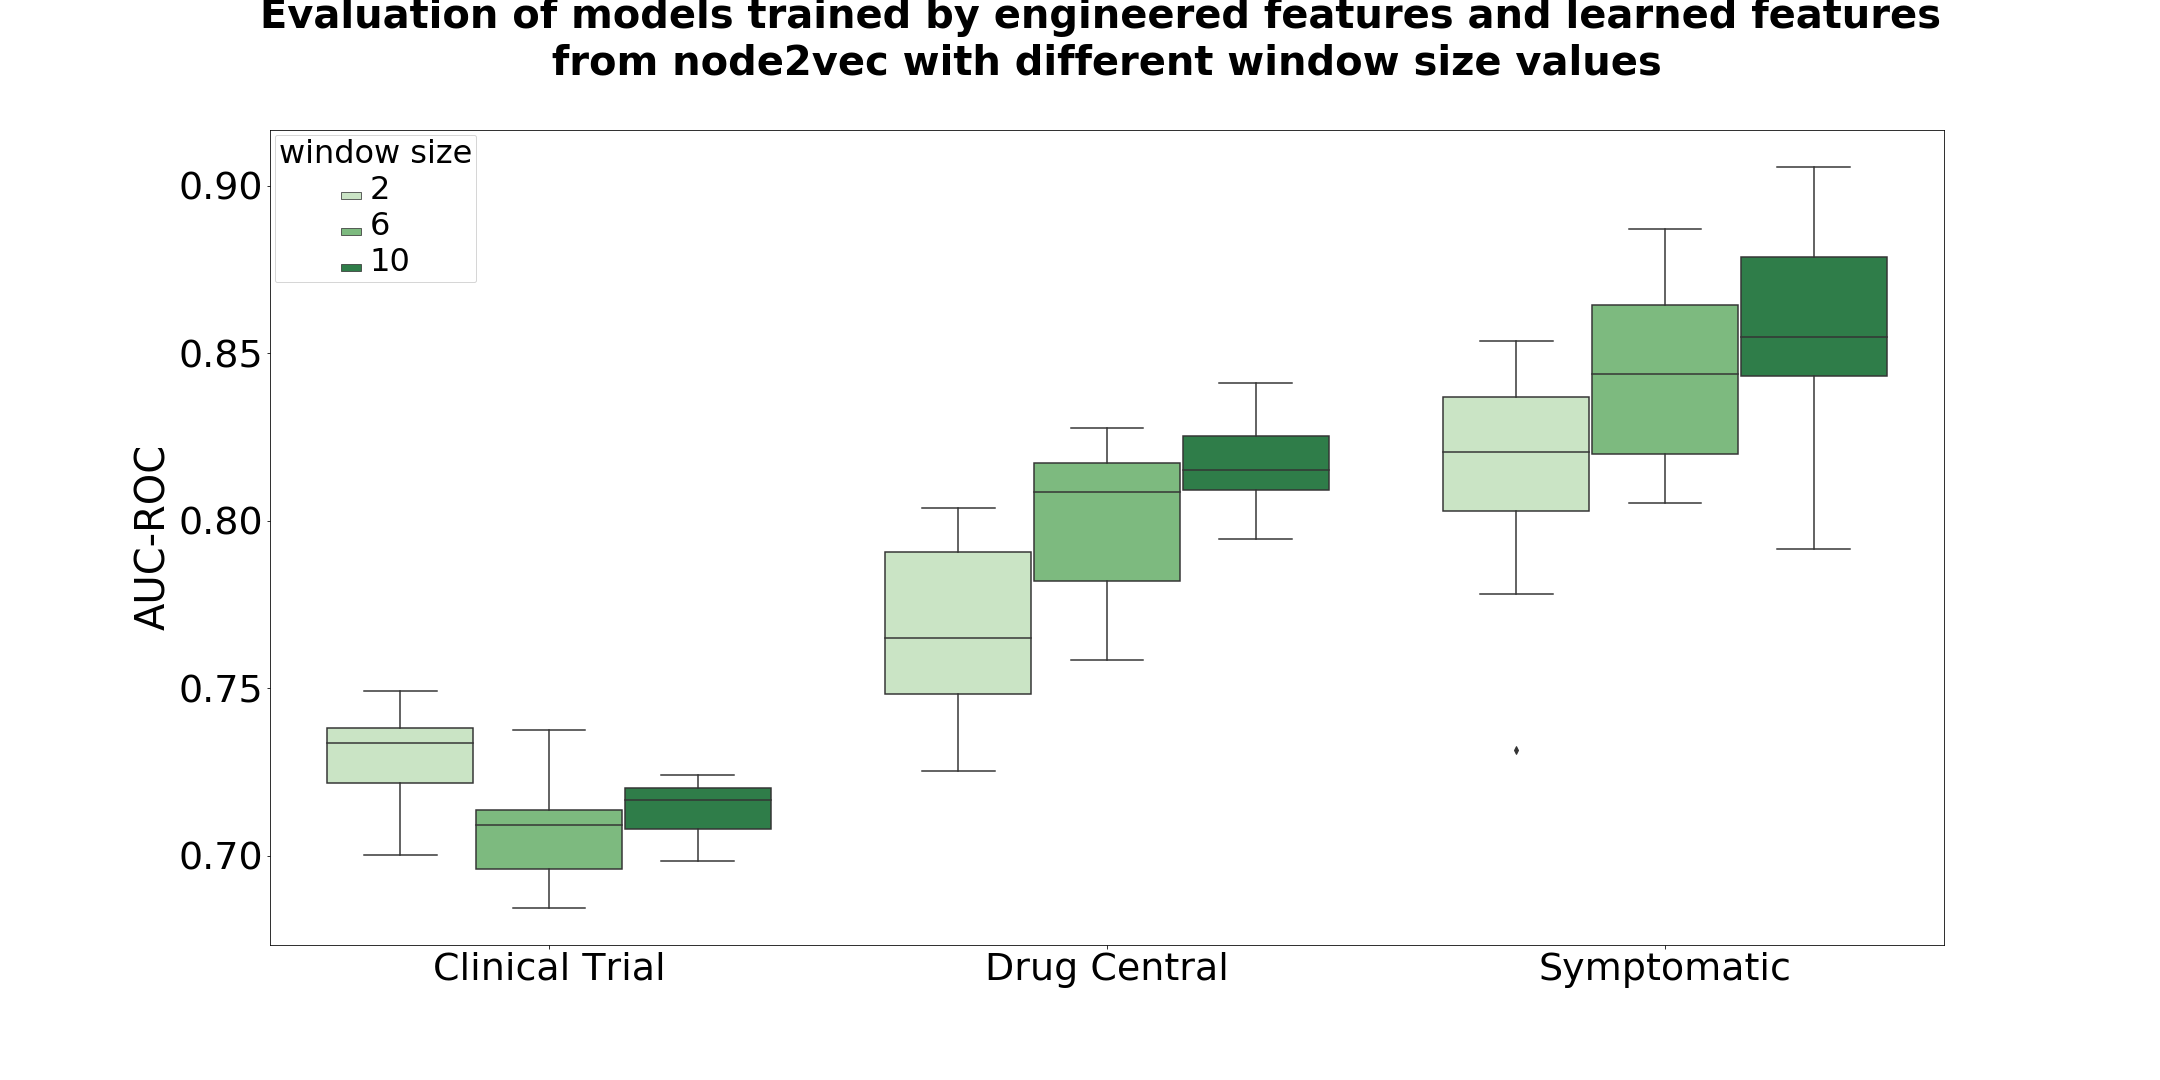
\includegraphics[scale=0.2]
    {figures/window_size.png}
    \captionsetup{justification=centering}
    \caption[Evaluation of different window\_size in node2vec]{\label{fig:window_size}Performance of logistic regression models with parameters: $p = 1$, $q = 1.0$, $repeat = 10$, $walk\_length = 30$, $window size = 2, 6, 10$, $number\_walk = 10$.
}
\end{figure}

The next step is to optimize \textit{p} and \textit{q}, As shown Figure \ref{fig:pq}, experiments are repeated ten times with same hyperparameters to test the robustness. Comparing performances of models to star signs (\ac{AUC-ROC} values of Rephetio), two data sets, Clinical Trial and Symptomatic give better evaluation results than Rephetio. Disease Modifying, the data set including training data, gives a smaller \ac{AUC-ROC} result with which shows that the models are less prone to be overfitting. Drug Central demonstrates comparable evaluation result to Rephetio. The comparison suggests that learned features can replace engineered features for building classification models with a better and more stable performance.

The performance of models improves with \textit{q} getting larger, suggesting that models with more local neighborhood information of the network are better than models with more global neighborhood information. This indicates that for a biological network, the local information like neighbors in small distance is more meaningful than that in large distance. In Rephetio work, the length of metapath is 2, 3 or 4, which is another indication that local information is comparatively more valuable than global information.

\begin{figure}[!h]
    \centering
    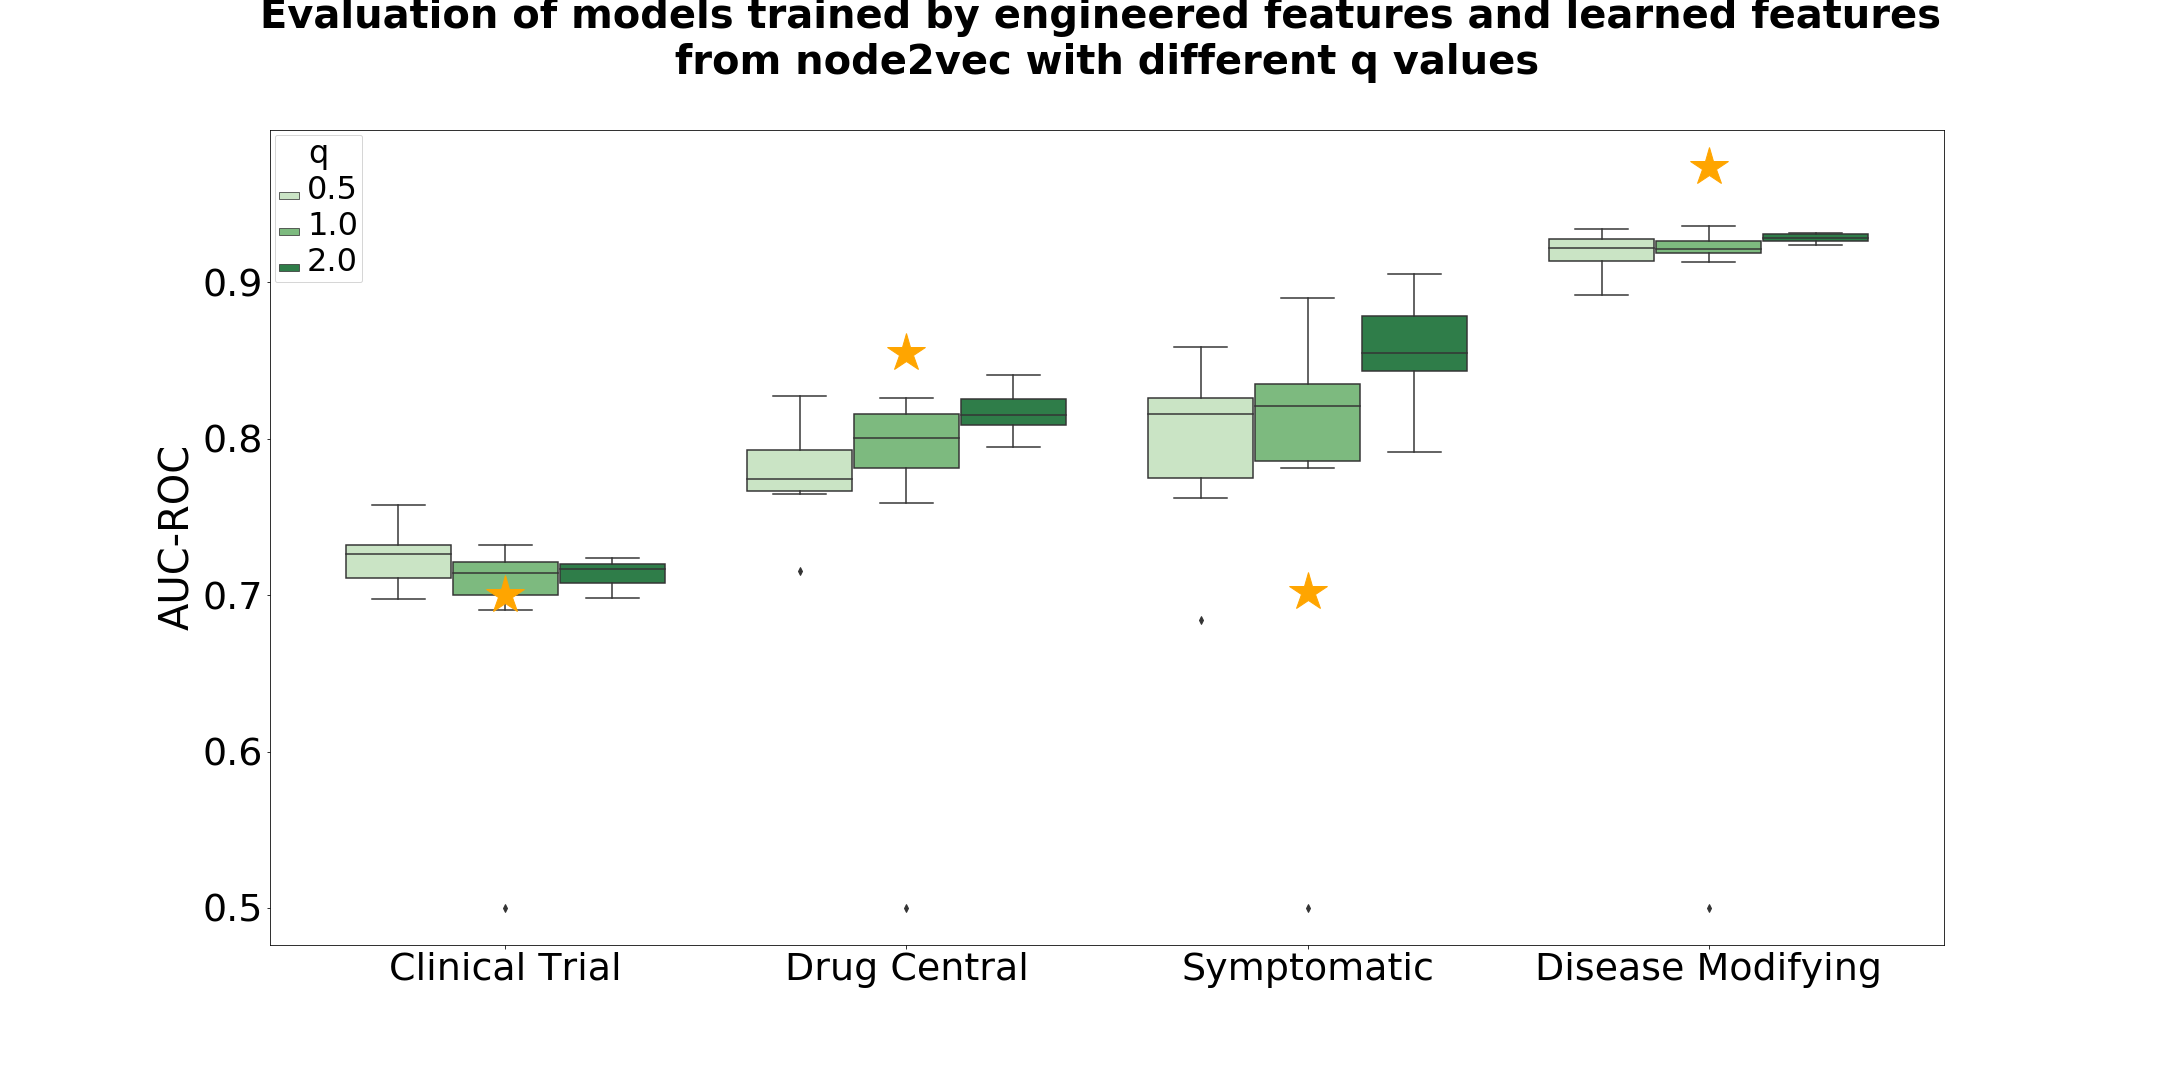
\includegraphics[scale=0.2]
    {figures/pq.png}
    \captionsetup{justification=centering}
    \caption[Evaluation of different q in node2vec]{\label{fig:pq}Performance of logistic regression models with parameters: $p = 1$, $repeat = 10$, $walk\_length = 30$, $window\_size = 10$, $number\_walk = 10$, $q =0.5, 1.0, 2.0$. Star signs are values of Rephetio.
}
\end{figure}

\textit{walk$\_$length} is the parameter to affect the length of walks. Larger \textit{walk$\_$length} makes random walk go through more nodes, then more neighbourhood information should be catched. As shown in Figure \ref{fig:wl}, it is obvious that the Symptomatic data set are getting narrower when walk length gets larger. It shows that larger \texit{walk\_length} makes the performance more stable, and the \ac{AUC-ROC} values of $walk\_length = 100$ are comparable with those of $walk\_length = 30, 50$. In this case, $p = 1$ and $q = 2$, make the random walk more local, and with walk\_length = 100, the random walk could explore over the local vicinity of the starting node. As a consequence, the performances of models tends to be similar because of the random walk catches similar and comprehensive information. For the other three data sets, changing of walk\_length doesn’t make much difference to the evaluation results.

\begin{figure}[!h]
    \centering
    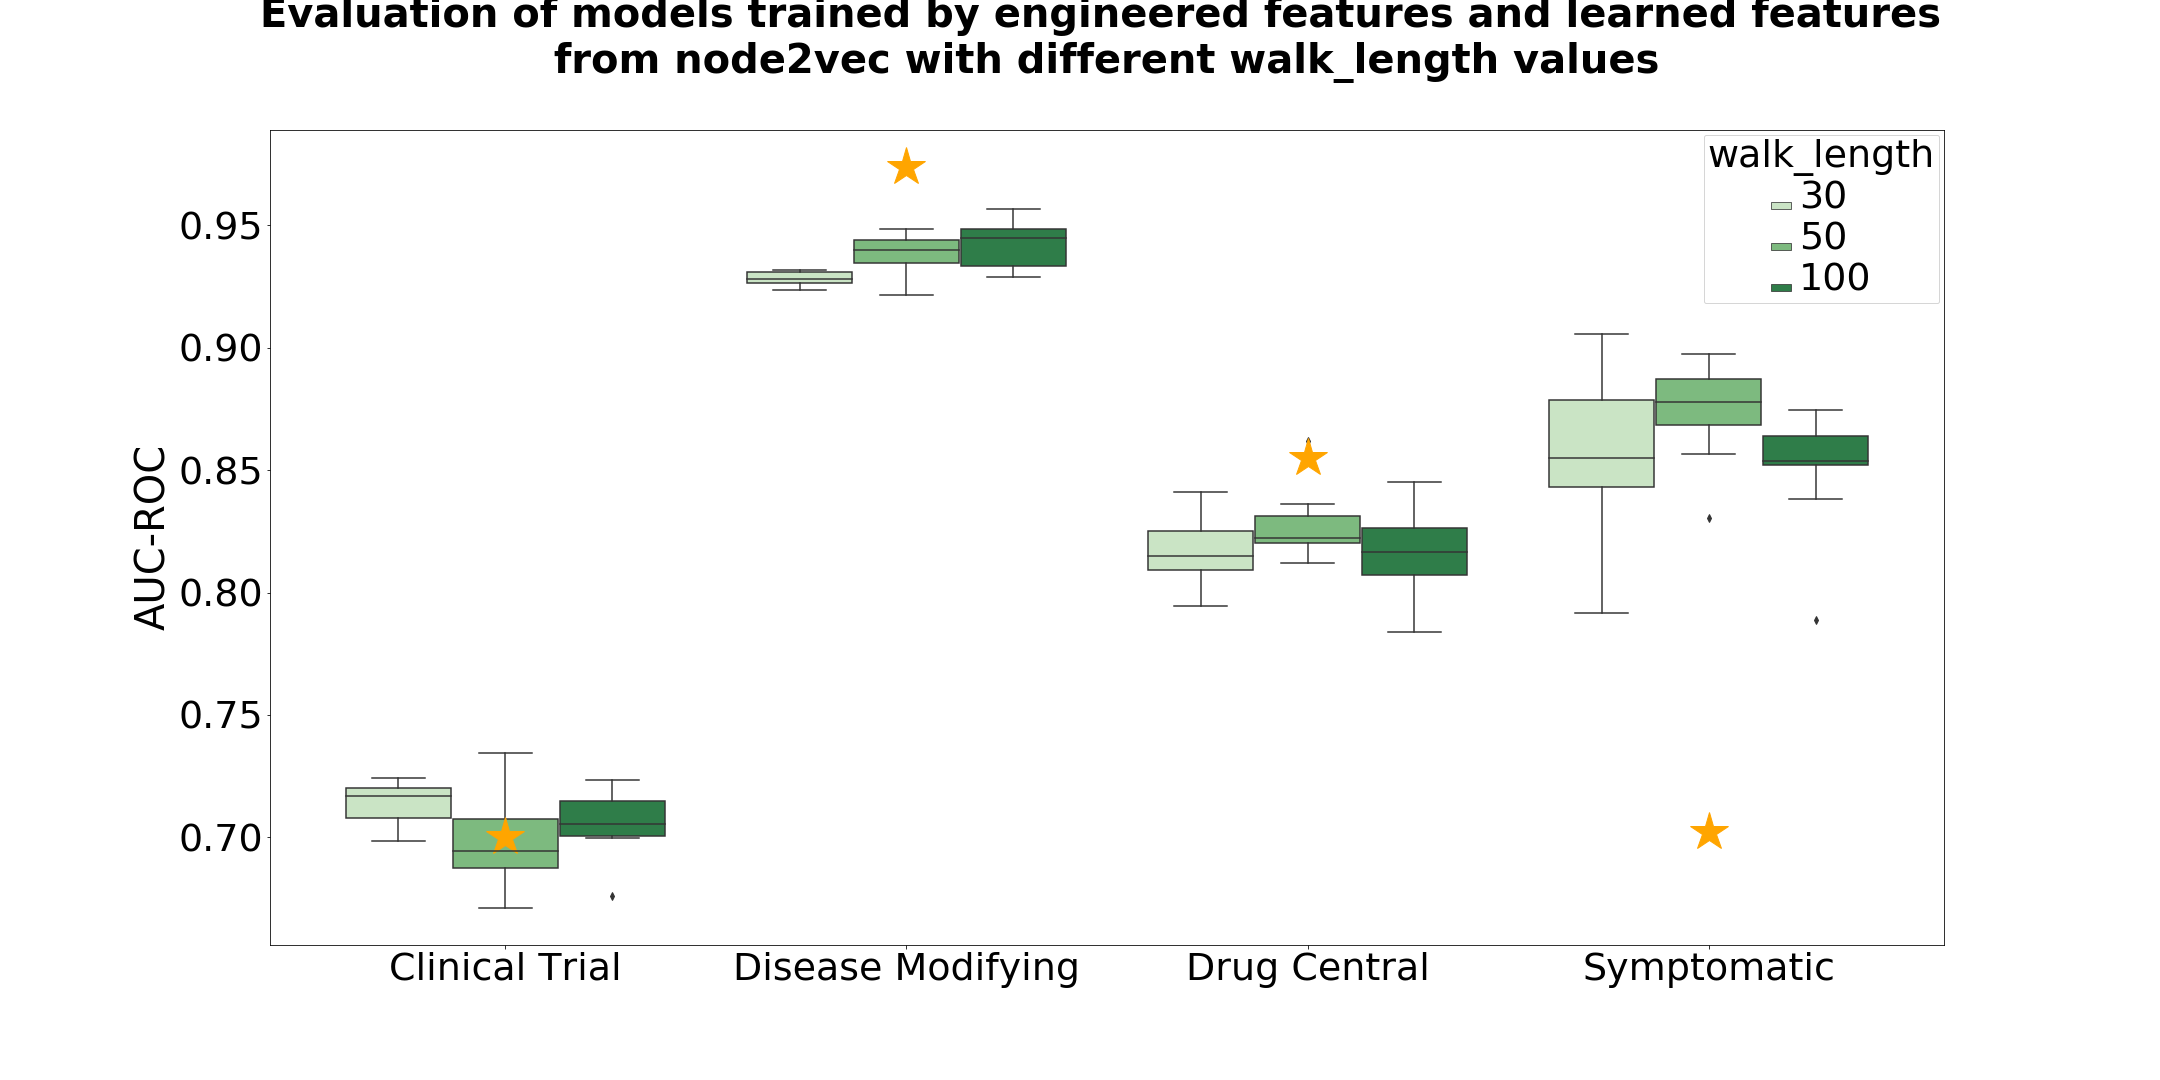
\includegraphics[scale=0.2]
    {figures/wl.png}
    \captionsetup{justification=centering}
    \caption[Evaluation of different walk\_length in node2vec]{\label{fig:wl}Performance Logistic regression models with parameters : $p = 1$, $q = 2$, $repeat = 10$, $window\_size = 10$, $number\_walk = 10$, $walk\_length = 30, 50, 100$. Star signs are values of Rephetio.
}
\end{figure}

AU-PR is more suitable for evaluating imbalanced data sets. As illustrated in Figure ~\ref{fig:node2vec_pr}, Two evaluation data sets (Clinical Trial and Symptomatic) show better results than Rephetio's.  In summary, learned features from node2vec can replace enginnered features in Rephetio, and learned features can perform better with an easy implementation. 

\begin{figure}[!h]
    \centering
    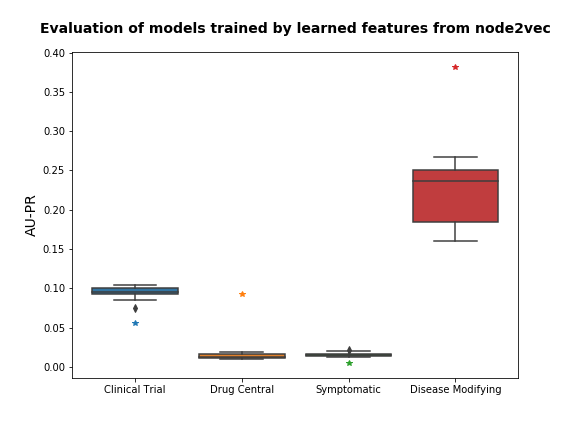
\includegraphics[scale=0.65]
    {figures/node2vec_pr.png}
    \captionsetup{justification=centering}
    \caption[AU-PRs of logistic regression models trained by learned features from node2vec]{\label{fig:node2vec_pr}Performance of logistic regression models with parameters : $p = 1$, $q = 2$, $repeat = 10$, $window\_size = 10$, $number\_walk = 10$, $walk\_length = 100$. Star signs are \ac{AU-PR} values of Rephetio.
}
\end{figure}

\subsection{Parameter Optimization of Edge2vec and Comparisons}

Edge2vec is improved from node2vec. The parameters of edge2vec are optimized based on the results of optimizing parameters of node2vec. But there are some unique parameters in edge2vec such as \textit{em\_iter} and \textit{max\_count} (discussed in section \ref{op_edge2vec}). \textit{em\_iter} controls the epochs of sampling the network to update \ac{TPM}, $em\_iter = 10$ is chosen. $max\_count$ is important for the quality of TPM, $max\_count = 10000$ is chosen. 

Another important parameter is the \textit{e\_step}, which controls the test function to evaluate correlation level between two edge types (explained in Table \ref{tab:tests in edge2vec}). As in node2vec, 10 times repeated experiments are operated to test the robustness of randomness with same parameters. 4 different tests, wilcoxon signed-rank ($e\_step =1$), entropy ($e\_step = 2$), pearson ($e\_step = 3$), spearman ($e\_step = 4$) are all tried in this thesis as shown in Figure \ref{fig:estep}. 

\begin{figure}[!h]
    \centering
    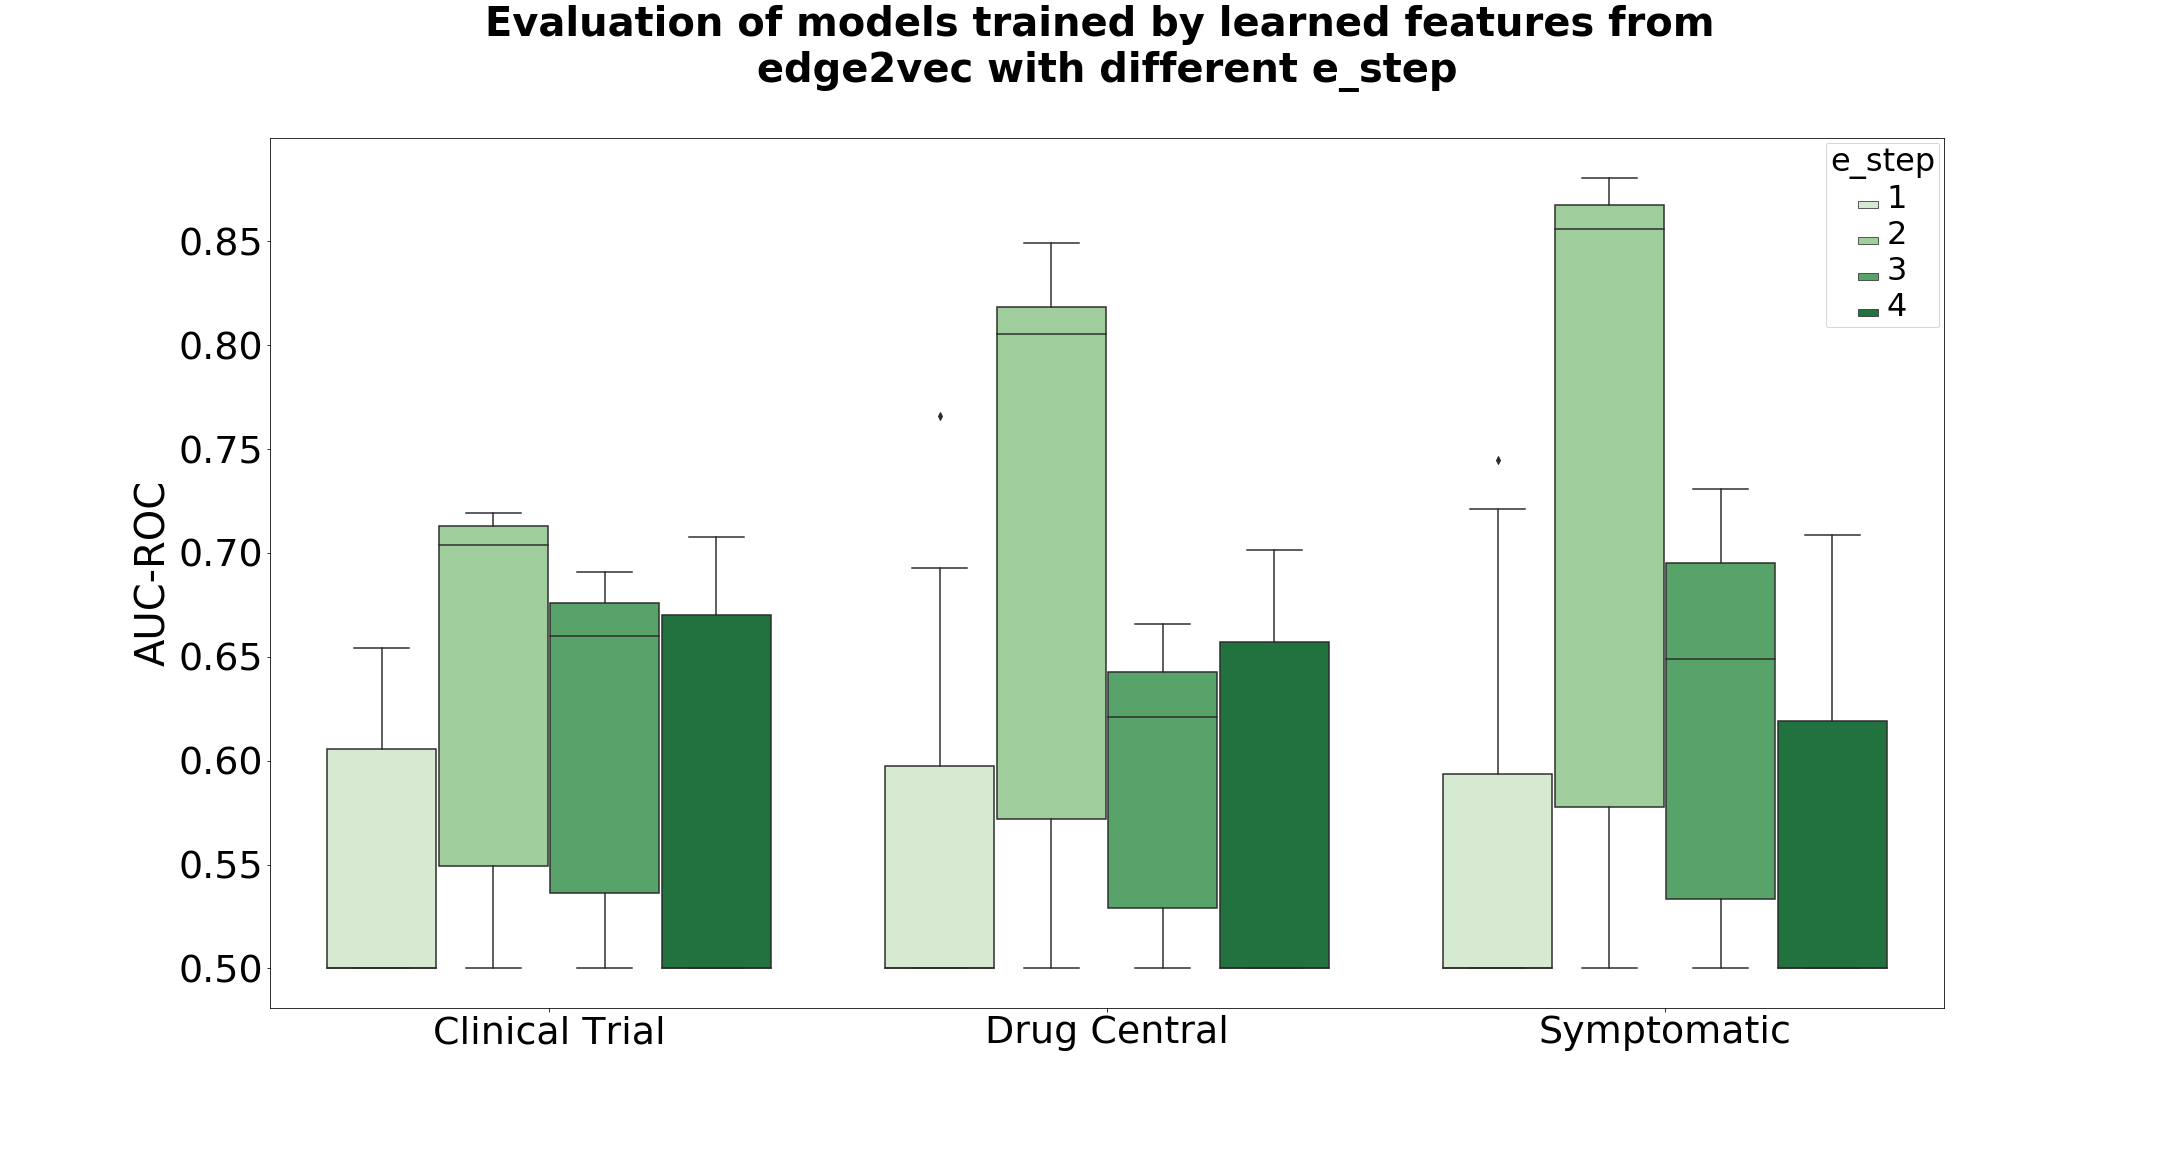
\includegraphics[scale=0.2]
    {figures/e_step.png}
    \captionsetup{justification=centering}
    \caption[Evaluation of different e\_step in edge2vec]{\label{fig:estep}Performance Logistic regression models with parameters : $p = 1$, $q = 1$, $repeat = 10$, $window\_size = 10$, $number\_walk = 10$, $walk\_length =  100$, $em\_iter = 10$, $max\_count = 10000$, $e\_step = 1, 2, 3, 4$
}
\end{figure}

The evaluation results of 4 tests all have high variance. The first test, wilcoxon signed-rank performs comparatively better than other three test functions. Further optimization should be done to control the high variance. Then \textit{window size} is changed to 3, in Figure \ref{fig:edge2vec_ws}, the evaluation results show that $window\_size = 3$ is more suitable for edge2vec applied in hetio, so $e\_step = 1$ and $window\_size = 3$ are chosen.

\begin{figure}[!h]
    \centering
    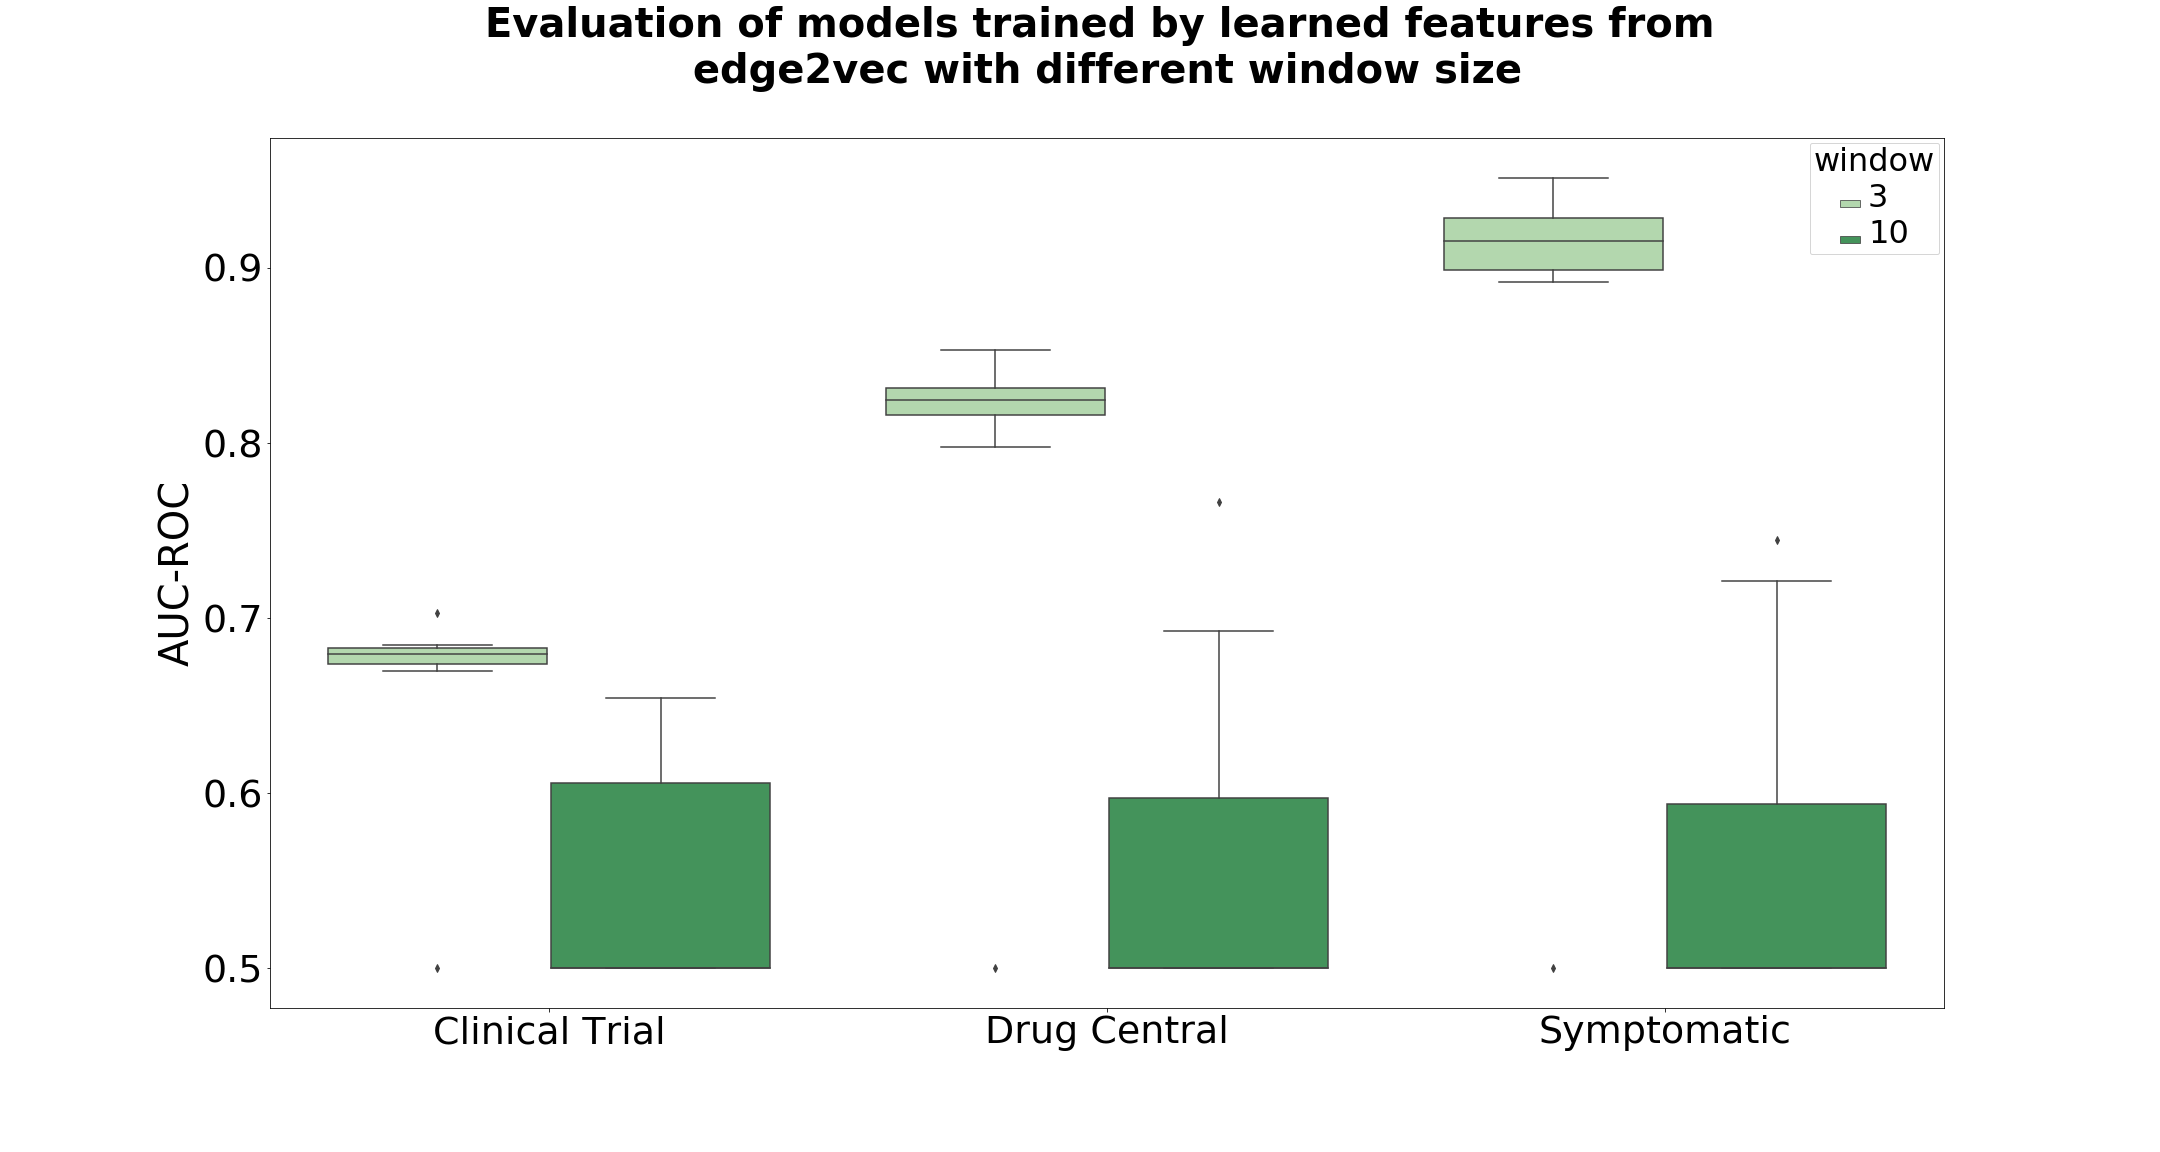
\includegraphics[scale=0.2]
    {figures/edge2vec_ws.png}
    \captionsetup{justification=centering}
    \caption[Evaluation of different window\_size in edge2vec]{\label{fig:edge2vec_ws}Performance Logistic regression models with parameters : $p = 1$, $q = 1$, $repeat = 10$, $window\_size = 3$, $number\_walk = 10$, $walk\_length =  100$, $em\_iter = 10$, $max\_count = 10000$. Star signs are values of Rephetio.
}
\end{figure}

As illustrated in Figure \ref{fig:edge2vec_roc}, comparing the performance of models to star signs (\ac{AUC-ROC} values of models from Rephetio), the evaluation results of Symptomatic data set surpass Rephetio's with a gap around 0.2. For the other three data sets, performances are comparable to Rephetio's. In Figure \ref{fig:edge2vec_pr}, \ac{AU-PR} values of Clinical Trial and Symptomatic of edge2vec outperform that of Rephetio. 

Symptomatic data set is from the same source of Disease Modifying (training data included). The outstanding performance of Symptomatic data set suggests that the learned feature vectors from edge2vec represent the network better than engineered features. Furthermore, the performances of 4 data sets of edge2vec are comparatively more stable than that of node2vec , which indicates that edge2vec performs better because it's able to capture the meaningful structure of the network with a more representative TPM for the network.

\begin{figure}[!h]
    \centering
    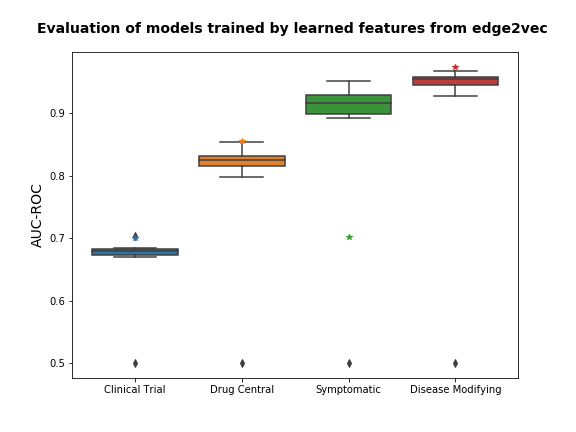
\includegraphics[scale=0.65]
    {figures/edge2vec_roc.png}
    \captionsetup{justification=centering}
    \caption[AUC-ROCs of logistic regression models trained by learned features from edge2vec]{\label{fig:edge2vec_roc}Performance of logistic regression models with parameters : $p = 1$, $q = 1$, $repeat = 10$, $window_size = 3$, $number_walk = 10$, $walk_length =  100$, $em\_iter = 10$, $max\_count = 10000$. Star signs are values of Rephetio.
}
\end{figure}

\begin{figure}[!h]
    \centering
    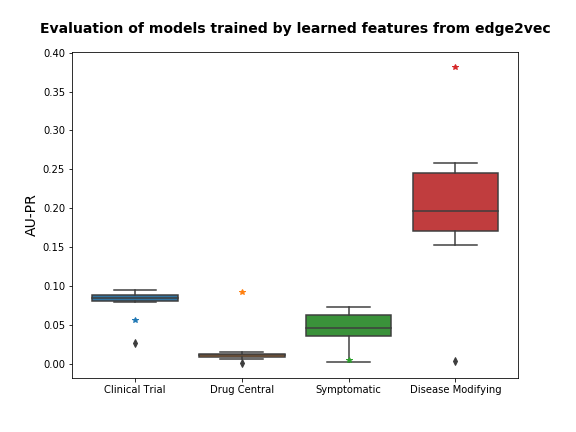
\includegraphics[scale=0.65]
    {figures/edge2vec_pr.png}
    \captionsetup{justification=centering}
    \caption[AU-PRs of Logistic regression models trained by learned features from edge2vec]{\label{fig:edge2vec_pr}Performance of logistic regression models with parameters : $p = 1$, $q = 2$, $repeat = 10$, $window\_size = 10$, $number\_walk = 10$, $walk\_length = 100$. Star signs are \ac{AU-PR} values of Rephetio.
}
\end{figure}

\subsection{Information of Classification Models with Best Performances}

To summary, models of best performance from Rephetio, node2vec, and edge2vec and their AUC-ROC values are presented in Table \ref{tab:AUCROC_table}. In Table \ref{tab:parameters_table}, parameters of chosen best performance models are presented. 

\begin{table}[!ht]
    \centering
    \begin{tabular}{|l|r|r|r|r|}
        \hline
        \textbf{} & \textbf{Clinical Trial} & \textbf{Drug Central} & \textbf{Symptomatic} & \textbf{Disease Modifying}\\
        \hline
        Rephetio & 0.700000 & 0.855000 & 0.702000 & 0.974000 \\
        \hline
        Node2vec & 0.714927 & 0.844998 & 0.852863 & 0.956823 \\
        \hline
        Edge2vec & 0.702855 & 0.829167 & 0.927183 & 0.967201\\
        \hline
    \end{tabular}
    \captionsetup{justification=centering}
    \caption{AUC-ROC values of chosen models}
    \label{tab:AUCROC_table}
\end{table}

\begin{table}[!ht]
    \centering
    \tiny
    \begin{tabular}{|l|r|r|r|r|r|r|l|r|r|r|}
        \hline
        \textbf{} & \textbf{num$\_$walk} & \textbf{walk$\_$length} & \textbf{window$\_$size} & \textbf{p} & \textbf{q} & \textbf{dimensions} & \textbf{operator} & \textbf{em$\_$iter} & \textbf{max$\_$count} & \textbf{e$\_$step}\\
        \hline
        Node2vec & 10 & 100 & 10 & 1 & 2 & 48 & Hadamard \\
        \hline
        Edge2vec & 10 & 100 & 3 & 1 & 1 & 48 & Hadamard & 10 & 10000 & 1 \\
        \hline
    \end{tabular}
    \captionsetup{justification=centering}
    \caption{Parameters of best performance models for node2vec and edge2vec}
    \label{tab:parameters_table}
\end{table}

\section{Predictions of Diseases for Vorinostat}

Vorinostat is a \ac{HDAC} inhibitor, affecting the \ac{HDAC} enzymes regulated the phenotypic and genotypic expression in cells in order to homeostasis and neoplastic growth. Apart from cutaneous T cell lymphoma the role of vorinostat for other types of cancers is being investigated ~\cite{bubna_vorinostat-overview_2015}. Because the affection of \ac{HDAC}s in neurodevelopment, memory formation, and cognitive processes, \ac{HDAC} inhibitors are expected to be novel agents neurodegenerative disorders such as \ac{AD}.

As shown in Table \ref{tab:vorinostat}, “probability” represents the probability of the prediction being true. Table \ref{tab:vorinostat} is sorted by the descending value of probability. \ref{fig:vorinastat} is generated from Drug Repurposing project in Hetionet, finding supportive paths between vorinostat and \ac{AD}.

\begin{table}[!ht]
    \centering
    \begin{tabular}{|p{4cm}|l|r|}
        \hline
        \textbf{Disease Ontology Identifier} & \textbf{Disease Name} & \textbf{Probability}\\
        \hline
        10652 & alzheimer's disease & 0.566710 \\
        \hline
        1312 & focal segmental glomerulosclerosis & 0.551427 \\
        \hline
        9744 & type 1 diabetes mellitus & 0.547426 \\
        \hline
        4159 & skin cancer & 0.543505 \\
        \hline
        10608 & celiac disease & 0.537503 \\
        \hline
        14330 & Parkinson's disease & 0.532105 \\
        \hline
        10976 & membranous glomerulonephritis & 0.528259 \\
        \hline
        332 & focal segmental glomerulosclerosis & 0.522691 \\
        \hline
        4989 & pancreatitis & 0.514514 \\
        \hline
    \end{tabular}
    \captionsetup{justification=centering}
    \caption{Part of repositioning prediction results of HDAC6 inhibitor, vorinostat}
    \label{tab:vorinostat}
\end{table}

As shown in Figure \ref{tab:vorinostat}, the ten most supportive path for vorinostat-\ac{AD} pair. \ac{HDAC} enzymes are keys to connect vorinostat and \ac{AD} ~\cite{desimone_histone_2019}. Rustenhoven et al. also suggest vorinostat could be a new drug for \ac{AD} due to its utility of limiting microglial-mediated inflammatory responses ~\cite{rustenhoven_pu.1_2018}. Figure \ref{tab:vorinostat} gives paths that vorinostat and memantine share the same side effects Thromboembolism and Squamous cell carcinoma, which could be another underlying mechanism that vorinostat could work in a similar way as memantine.

\begin{figure}[!h]
    \centering
    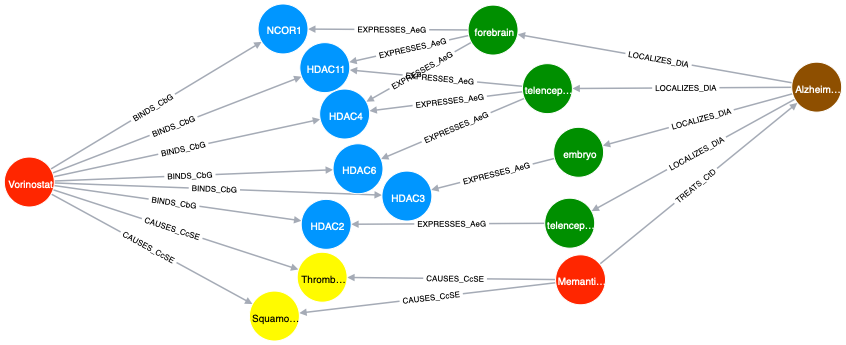
\includegraphics[scale=0.5]
    {figures/vorinastat.png}
    \captionsetup{justification=centering}
    \caption{\label{fig:vorinastat} Ten most supportive paths connecting vorinostat and Alzheimer’s disease
}
\end{figure}

The highest probability of prediction for vorinostat is colon cancer. And the probability of vorinostat - AD pair is not high, which is reasonable because HDAC-6 is most relevant to cancers based on studies and researches until now, AD and Parkinson’s disease are predicted to have an edge with vorinostat with a comparatively low but still positive probability, which suggests that the model is able to catch information of graph and give convincing predictions.

\section{Predictions of Drugs for Alzheimer’s Disease}

Table \ref{tab:alzheimer} shows ten of the drug candidate predictions for AD. 

\begin{table}[!ht]
    \centering
    \begin{tabular}{|p{6cm}|l|r|}
        \hline
        \textbf{DrugBank Compound ID} & \textbf{Compound Name} & \textbf{Probability}\\
        \hline
        DB06287 & Temsirolimus & 0.90302 \\
        \hline
        DB00193& Tramadol & 0.89986 \\
        \hline
        DB00715 & Paroxetine & 0.89033 \\
        \hline
        DB00877 & Sirolimus & 0.88865 \\
        \hline
        DB00724 & Imiquimod & 0.85494 \\
        \hline
        DB00285 & Venlafaxine & 0.85105 \\
        \hline
        DB08828 & Vismodegib & 0.84252 \\
        \hline
        DB00494 & Entacapone & 0.82564 \\
        \hline
        DB00289 & Atomoxetine & 0.82018 \\
        \hline
        DB00996 & Gabapentin & 0.81912 \\
        \hline
    \end{tabular}
    \captionsetup{justification=centering}
    \caption{Part of predictions for Alzheimer’s disease}
    \label{tab:alzheimer}
\end{table}

Temsirolimus is an inhibitor of mammalian target of rapamycin (mTOR) kinase, a component of intracellular signaling pathways involved in the growth and proliferation of cells ~\cite{schmelzle_tor_2000}. It was approved by \ac{FDA} in 2007 to be used for metastatic renal-cell carcinoma ~\cite{hudes_temsirolimus_2007}. Jiang et al. found that temsirolimus promotes autophagic clearance of amyloid-$\beta$ and provides protective effects in cellular and animal models of \ac{AD} ~\cite{jiang_temsirolimus_2014}. Christelle et al. also suggested that temsirolimus was able to alleviate tau pathology in mutant tau transgenic mice ~\cite{frederick_rapamycin_2015}. As illustrated in Figure \ref{fig:temsirolims}, the underlying mechanism might be that temsirolimus affects PPP3CA, and PPP3CA can alter the sensitivity of animals to electrophysiological and cognitive impairments caused by amyloid-$\beta$ exposure ~\cite{nicholls_pp2a_2016}. The third ranking drug is paroxetine, which was researched that it lowers intracellular APP while maintaining APLP-1 levels ~\cite{payton_drug_2003}, which could be the underlying mechanism of paroxetine connecting to \ac{AD}.

\begin{figure}[!h]
    \centering
    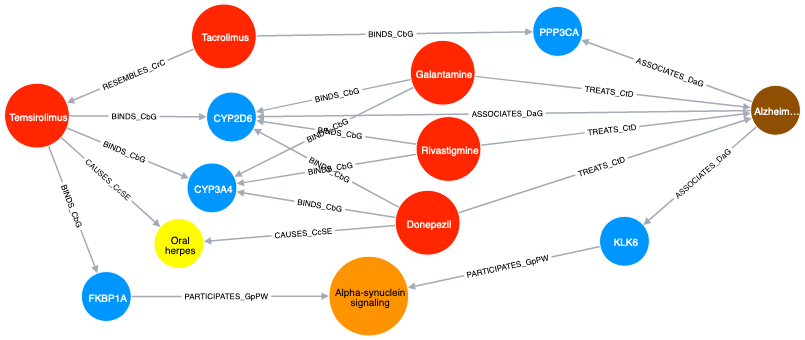
\includegraphics[scale=0.5]
    {figures/temsirolims.png}
    \captionsetup{justification=centering}
    \caption{\label{fig:temsirolims}Ten most supportive metapaths connecting temsirolimus and Alzheimer’s Disease. Temsirolimus-resembles-Tacrolimus-binds-PPP3CA-associates-Alzheimer's Disease is the path having supportive researching evidence.
}
\end{figure}

In conclusion, network is a data structure good for applying computational algorithms and visualization. The work of this thesis indicates that node2vec and edge2vec are powerful \ac{NRL} methods for generating high-quality feature vectors from networks to train downstream machine learning models in order to conduct drug repositioning tasks. And compared with engineered features, the advantages of learned features are simple implementation and making machine learning models more generalizable.Therefore, learned features can replace engineered features for drug repositioning tasks with a better performance with one set of optimized parameters. 